\documentclass{classrep}
\usepackage{polski}
\usepackage{ucs}
\usepackage[utf8x]{inputenc}
\usepackage[T1]{fontenc}
\usepackage{cite}
%\usepackage{tcolorbox}
%\usepackage{apacite}
\usepackage{cancel}
\usepackage{graphicx}
\usepackage{dcolumn}
\usepackage{color}
\usepackage{colortbl}
\usepackage{enumerate}
\usepackage{url}
\usepackage[squaren]{SIunits}
\usepackage{icomma}
\usepackage{hyperref}
%\usepackage{url}
\usepackage{float}
\usepackage{indentfirst}
\usepackage{amssymb}
\usepackage{verbatim}
\usepackage{tabulary}
\usepackage{longtable}
\usepackage{rotating}
\usepackage{formular}
\usepackage{marginnote}
\usepackage{listingsutf8}
\usepackage{ifpdf}
%\usepackage{natbib}
\usepackage{fancybox}
\lstset{inputencoding=utf8/latin2,breaklines=true}
\newFRMfield{wyraz}{2cm}
\newif\ifShowAnswers
%\ShowAnswerstrue
\newcommand{\fillin}[2]{\ifShowAnswers{#1}\else{\marginnote{#2}\useFRMfield{wyraz}}\fi}
\newtheorem{xdefinicja}{Definicja}
\newenvironment{definicja}{\begin{xdefinicja}\normalfont}{\end{xdefinicja}}
\ifpdf
\newcommand{\obraz}[3]{
\begin{figure}[H]
\centering
\includegraphics[width=9cm]{#1.pdf}
\caption{#3}
\label{fig:#2}
\end{figure}
}
\newcommand{\malyobraz}[3]{
\begin{figure}[H]
\centering
\includegraphics[width=4cm]{#1.pdf}
\caption{#3}
\label{fig:#2}
\end{figure}
}
\newcommand{\podwojnyobraz}[4]{
\begin{figure}[H]
\centering
\includegraphics[width=4cm]{#1.pdf}
\includegraphics[width=4cm]{#2.pdf}
\caption{#4}
\label{fig:#3}
\end{figure}
}
\newcommand{\poziomyobraz}[2]{
\begin{sidewaysfigure}
\centering
\includegraphics[width=25cm]{#1.pdf}
%\caption{#2}
\label{fig:#2}
\end{sidewaysfigure}
}
\else
\newcommand{\obraz}[3]{
\begin{figure}[H]
\centering
\includegraphics[width=9cm]{#1.eps}
\caption{#3}
\label{fig:#2}
\end{figure}
}
\newcommand{\malyobraz}[3]{
\begin{figure}[H]
\centering
\includegraphics[width=4cm]{#1.eps}
\caption{#3}
\label{fig:#2}
\end{figure}
}
\newcommand{\podwojnyobraz}[4]{
\begin{figure}[H]
\centering
\includegraphics[width=4cm]{#1.eps}
\includegraphics[width=4cm]{#2.eps}
\caption{#4}
\label{fig:#3}
\end{figure}
}
\newcommand{\poziomyobraz}[2]{
\begin{sidewaysfigure}
\centering
\includegraphics[width=25cm]{#1.eps}
%\caption{#2}
\label{fig:#2}
\end{sidewaysfigure}
}
\fi
\newcommand{\rysunek}[4]{
\begin{figure}[H]
\centering
\begin{picture}#3
#4
\end{picture}
\caption{#2}
\label{fig:#1}
\end{figure}
}
\newcommand{\tabela}[4]{
\begin{table}[H]
\centering
\begin{tabular}[t]{#3}
#4
\end{tabular}
\caption{#2}
\label{tab:#1}
\end{table}
}

\newcommand{\tabelap}[4]{
\begin{table}[p]
\centering
\begin{tabular}[t]{#3}
#4
\end{tabular}
\caption{#2}
\label{tab:#1}
\end{table}
}

\newcommand{\tabelah}[4]{
\begin{table}[ht]
\centering
\begin{tabular}[t]{#3}
#4
\end{tabular}
\caption{#2}
\label{tab:#1}
\end{table}
}

\newcommand{\tabelat}[4]{
\begin{table}[t]
\centering
\begin{tabular}[t]{#3}
#4
\end{tabular}
\caption{#2}
\label{tab:#1}
\end{table}
}

\newcommand{\tabelab}[4]{
\begin{table}[b]
\centering
\begin{tabular}[t]{#3}
#4
\end{tabular}
\caption{#2}
\label{tab:#1}
\end{table}
}

\newcommand{\ltabela}[3]{
\clearpage
\begin{longtable}[c]{#2}
\caption{#1}\\
#3
\end{longtable}
}

\lstdefinelanguage{Smalltalk}{
  morekeywords={true,false,self,super,nil},
  sensitive=true,
  morecomment=[s]{"}{"},
  morestring=[d]',
}
\lstdefinestyle{SmalltalkStyle}{
  literate={:=}{{$\gets$}}1{^}{{$\uparrow$}}1
} 

\usepackage{amsfonts}
\usepackage[intlimits]{amsmath}


\studycycle{Informatyka, studia dzienne}
\coursesemester{III}

\coursename{Pracownia Problemowa}
\courseyear{2014}

\courseteacher{dr. inż Aneta Poniszewska-Marańda}
\coursegroup{poniedziałek, 14:15}

\author{%
  \studentinfo{Mateusz Grotek}{186816} \and
  \studentinfo{Mateusz Jakóbczak}{186819} \and
  \studentinfo{Rafał Jurkiewicz}{186822} \and
  \studentinfo{Łukasz Kotyński}{186829} \and
  \studentinfo{Paweł Tarasiuk}{186875}
}

\title{Kontrola dostępu w dynamicznych systemach informatycznych}

\begin{document}
\maketitle

\section{Problem}
Przedstawiony problem dotyczy tworzenia i analizy zaawansowanych, inteligentnych mechanizmów kontroli dostępu w dynamicznych systemach informatycznych. Celem projektu jest
zapoznanie się ze stosowanymi rozwiązaniami, zdobycie aktualnej wiedzy na ten temat, a także wykonanie praktycznej implementacji wybranych rozwiązań.
\section{Wprowadzenie}
Pierwszą rzeczą, jaką należy zrobić w celu rozwiązania postawionego werbalnie problemu jest dokładne zrozumienie określeń użytych w jego specyfikacji. W wypadku
kontroli dostępu w dynamicznych systemach informatycznych istotną rzeczą jest zwrócenie uwagi na pojęcia kontroli dostępu i dynamicznego systemu informatycznego. Jako, że główna
część zagadnienia skupia się na zapewnieniu kontroli dostępu, wyjaśnimy najpierw drugie, mniej istotne pojęcie, jakim są dynamiczne systemy informatyczne.

Pojęcie dynamiki można tutaj
rozumieć na różne sposoby, ale na pewno podstawowym aspektem jest tutaj wrażliwość na zmieniające się warunki, takie jak na przykład czas, lub pewne zdarzenia zachodzące zarówno 
w samym systemie, jak i poza nim. Oznacza to, że system nie powinien robić żadnych założeń na temat tego co się aktualnie dzieje, a raczej reagować dynamicznie. Dla porównania
możemy wskazać na przykład dostęp do plików na serwerze. Rozwiązanie statyczne mogłoby polegać na przykład na tym, że w systemie jest na stałe zapamiętane (zaszyfrowane) hasło,
które użytkownik musi podać przy logowaniu, po którym uzyskuje pełny i nieograniczony czasowo dostęp do pewnych, na sztywno zdefiniowanych zasobów, takich jak pewne pliki w pewnych katalogach.
Skontrastujmy to z systemem w którym dostęp do plików jest ograniczony pod względem na przykład ilości osób, które jednocześnie z nich korzystają, przy czym czas korzystania może być ograniczony
w zależności od konkretnej osoby, a także od ilości osób. Poza tym dostęp może być włączany konkretnym osobom w konkretnych godzinach. Co więcej, uzyskanie dostępu może zależeć od
wydania zezwolenia. Jak widać stworzenie systemu dynamicznego jest dużo trudniejsze od stworzenia systemu statycznego.

Wróćmy teraz do pojęcia kontroli dostępu. Kontrola dostępu oznacza, że dostęp do pewnych zasobów jest, z jednej strony, dozwolony lub zabroniony, natomiast z drugiej, że
jest on nadzorowany, czyli że na przykład każde skorzystanie z zasobów jest zapisywane, lub nawet zatwierdzane przez odpowiednią osobę. Wynika z tego, że elementami kontroli
dostępu są nie tylko autentykacja i autoryzacja, ale także wydawanie zgody na dostęp i audyt.
\section{Aktualny stan wiedzy}
Jest wiele różnych sposobów na zapewnienie kontroli dostępu. Co więcej sposoby te niekoniecznie kolidują ze sobą, a często mogą ze sobą współpracować. Do podstawowych mechanizmów
mogących zapewnić kontrolę dostępu należą\cite{owasp}\cite{computer}\cite{wikibooks}:
\begin{itemize}
\item kontrola dostępu uznaniowa \textit{Discretionary Access Control, DAC}
\item kontrola dostępu obowiązkowa \textit{Mandatory Access Control, MAC}
\item kontrola dostępu oparta na rolach \textit{Role Based Access Control, RBAC}.
\end{itemize}
Każdy z tych modeli różni się elementem, który przydziela prawa dostępu, a także mechanizmami dostępu\cite{wikibooks}. 

W przypadku \textbf{DAC} zarządzaniem uprawnieniami zajmują się właściciele danych. Często wykorzystywane są do tego listy kontroli dostępu (\textit{Access Control Lists, ACLs}).
Dobrym przykładem takiego rozwiązania jest dostęp do plików i katalogów na dysku w Uniksie/Linuksie. Właściciel pliku/katalogu może ustawić prawa dostępu dla siebie, grupy, do której należy
dany plik, a także dla osób spoza grupy. Prawa te, to prawa odczytu, zapisu i wykonywania, a także pewne dodatkowe prawa o których nie będziemy tutaj pisać. Jednoczesną zaletą i wadą takiego
rozwiązania jest fakt, że zarządzanie uprawnieniami dokonywane jest przez właścicieli zasobów. Jest to zaleta, gdyż łatwo jest zarządzać właścicielowi zasobami, które tylko on posiada,
gdyż ich ilość jest ograniczona. Jest to wada, gdyż brak jest centralnego nadzoru nad uprawnieniami.

Przypadek \textbf{MAC} zakłada, że przydzielaniem uprawnień zajmuje się sam system na podstawie etykiet przydzielonych do osób i zasobów. Na przykład jeśli osoba ma przydzieloną
etykietę ,,Secret'', to może ona przeglądać zasoby oznaczone jako ,,Secret'', a także zasoby na poziomach niższych. Nie może już za to przeglądać zasobów oznaczonych jako ,,Top Secret''.
Sam system zapewnia dostęp do zasobów na podstawie ustalonej w trakcie jego tworzenia polityki bezpieczeństwa.

Przypadek \textbf{RBAC} bazuje na przydzieleniu dla każdego użytkownika jego roli w organizacji. Przydzielaniem ról i uprawnień do ról zajmuje się administrator. Następnie każdej roli
są przydzielane dostępne dla niej zasoby.

Amerykańskie ministerstwo obrony (DoD) zdefiniowało w dokumencie Trusted Computer System Evaluation Criteria\cite{TCSEC} (w skrócie TCSEC) następujące 4 poziomy dostępu:
\begin{itemize}
\item A -- ochrona zweryfikowana
\item B -- ochrona obowiązkowa
\item C -- ochrona uznaniowa
\item D -- ochrona minimalna
\end{itemize}

Ochrona minimalna dotyczy systemów, które zostały ocenione, ale nie spełniły żadnych kryteriów. Kolejne poziomy oznaczają lepszą ochronę. W wypadku poziomu C możliwa jest
tylko ochrona DAC. Dla poziomu B mamy także politykę ochrony, czyli dodatkowo MAC. W wypadku A procedury zostały formalnie zweryfikowane (np. przez podanie dowodu poprawności programu).

W naszym projekcie postanowiliśmy użyć połączenia modeli RBAC i MAC. Z modelu RBAC weźmiemy pojęcie roli. Każdy użytkownik będzie przypisany do określonej roli, której przysługują
określone uprawnienia. Jednakże nie będą to uprawnienia statyczne, ale dynamiczne, co oznacza, że w pewnych warunkach pewne uprawnienia będą nieważne lub ograniczone.
W tym celu zastosowane zostaną elementy modelu MAC. Inaczej mówiąc model RBAC będzie miał za zadanie zapewnić pewne statyczne uprawnienia, które następnie będą modyfikowane dynamiczne
przez odpowiednie zdarzenia zachodzące w systemie i poza nim. Oznacza to, że nasz system uprawnień będzie miał strukturę dwuwarstwową. Pierwszą warstwę będą stanowić
przypisane przez administratora systemu role i ich uprawnienia. Nazwijmy takie uprawnienia \textbf{możliwościami} roli. To że rola ma możliwość nie oznacza automatycznie,
że ma ona także \textbf{uprawnienie}. Zdecyduje o tym system na podstawie aktualnych zdarzeń.

Model RBAC został wstępnie opisany w artykule Ferraiolo i Kuhna\cite{RBAC}, a dalsze szczegóły można znaleźć w artykule Sandhu, Ferraiolo i Kuhna\cite{NISTModel}.
Amerykański Narodowy Instytut Standardów i Technologii (National Institute of Standards and Technology) opracował model\cite{NIST}, którego celem jest standaryzacja systemów
bazujących na rolach. Role stanowią element pośredni, ułatwiający zarządzanie. Do jednej roli może być przyporządkowana więcej niż jedna osoba. Ponadto do jednej roli mogą być
przyporządkowane różne zasoby.

Standard NIST podzielił systemy RBAC na 4 klasy, przy czym każda następna klasa jest rozszerzeniem poprzedniej:
\begin{itemize}
\item płaski RBAC
\item hierarchiczny RBAC
\item RBAC z więzami
\item symetryczny RBAC
\end{itemize}
Najprostszą odmianą jest płaski RBAC, który zawiera powiązania między rolami a użytkownikami i uprawnieniami. RBAC hierarchiczny dodatkowo zawiera powiązania między rolami,
takie jak na przykład dziedziczenie. W RBAC z więzami dodatkowo jest zapewniona spójność ról i podział odpowiedzialności, a także ograniczenia na powiązania między użytkownikami
i rolami, a także pomiędzy jedną rolą a drugą. W symetrycznym RBAC dodatkowo jest możliwość nakładania ograniczeń na powiązania między rolami a uprawnieniami. Jest także możliwość przeglądania
i zaawansowanego zarządzania uprawnieniami.

Nasz system chcemy zrealizować jako system z uprawnieniami bazującymi na regułach. Silniki reguł biznesowych to popularne rozwiązanie w firmach. Służą tam one na przykład to zarządzania
przepływem dokumentów, a także zarządzania zasobami ludzkimi. Najpopularniejszym rozwiązaniem jest Drools\cite{Drools}, który jest systemem reguł przeznaczonym dla środowiska Java i rozwijanym
przez firmę RedHat. Jednakże w naszym projekcie chcemy użyć innego sprawdzonego rozwiązania, jakim jest język Prolog\cite{Prolog}. Jest to język programowania deklaratywnego w logice,
który jest bardzo dobrze dostosowany do rozwiązywania skomplikowanych problemów w których występuje wiele reguł. 
\section{Opis rozwiązania problemu}
Jak opisaliśmy powyżej, aby zapewnić naszemu rozwiązaniu maksymalną elastyczność zastosowaliśmy reguły opisane jako reguły Prologowe. Dzięki temu możliwe stało się dowolne ustalenie zależności
między uprawnieniami. Zastosowaliśmy model oparty o role, jednakże nasz system pozwala także przypisywać uprawnienia bezpośrednio konkretnym użytkownikom. Co więcej można zupełnie
dowolnie kształtować zależności między rolami. Na przykład osobie posiadającej rolę administratora można automatycznie przypisać rolę wikipedysty itp.

Omówiliśmy powyżej sposób organizacji zarządzania uprawnieniami. Jednakże uprawnienia służą przecież do zarządzania określonymi zasobami. Optymalnym rozwiązaniem jest
zdefiniowanie ogólnej postaci zasobu, i umożliwieniu zarządzania uprawnieniami do niej. Dzięki postawieniu problemu na takim poziomie ogólności byliśmy w stanie oddzielić proces
definiowania i zarządzania uprawnieniami, od procesu tworzenia zasobów. Dzięki temu nasz system uprawnień można dopasować praktycznie do dowolnych zasobów, które jesteśmy w stanie
przedstawić w określonej postaci ogólnej. 

Aby omówić tą postać ogólną należy zauważyć, że każdy zasób, aby był dostępny dla użytkownika za pomocą strony internetowej, musi mieć przypisany mu określony widok, za pomocą którego użytkownik
wchodzi w interakcję z tym zasobem. Podstawowymi operacjami, jakie można wykonać na zasobie są operacje czytania zasobu i zapisywania zasobu. Wszystkie inne operacje można
rozumieć jako pewne wersje tych dwóch operacji. Jako przykład podamy chociażby dostęp do kolekcji zasobów. Dodawanie elementu do kolekcji to po prostu pisanie do kolekcji.
Przeglądanie listy zasobów w kolekcji to odczyt z kolekcji. Tworząc odpowiednią ilość zasobów i bazując na tych dwóch operacjach jesteśmy w stanie opisać praktycznie dowolny zasób.

W związku z powyższym każdą interakcje użytkownika z zasobem możemy opisać za pomocą czterech parametrów zasobu i dwóch parametrów użytkownika:
\begin{itemize}
  \item parametry zasobu:
  \begin{itemize}
    \item unikalny identyfikator zasobu
    \item typ zasobu
    \item unikalny identyfikator widoku
    \item typ widoku
  \end{itemize}
  \item parametry użytkownika
  \begin{itemize}
    \item nazwa użytkownika
    \item hasło
  \end{itemize}
\end{itemize}

Używając tych danych możemy już zaproponować pewien system kontroli dostępu. Jednakże system taki byłby niepełny, gdyż nie możliwe byłoby w nim zdefiniowanie zależności od innych
parametrów systemu w aktualnym jego stanie. Dlatego nasz system umożliwia dostęp do dowolnego beana z poziomu Prologu. Dzięki takiemu rozwiązaniu możemy na bieżąco podczas weryfikacji
uprawnień odpytywać dowolne elementy systemu o ich stan.

\section{Opis implementacji}

Implementacja rozwiązania problemu została wykonana na platformie JavaEE w technologii JSF i PrimeFaces. Początkowo planowaliśmy użyć bazy danych, jednakże w toku prac okazało się,
że takie rozwiązanie jest zbędne i wprowadziłoby tylko niepotrzebne komplikacje. Co więcej nasz system powinien być dostępny dla dowolnych rozwiązań technologicznych, także takich, które nie
zawierają bazy danych.

Każdy moduł jest niezależnym komponentem wykonanym przy użyciu technologii JSF Compound Components.
Lista komponentów jest przedstawiona na rysunku \ref{fig:komponenty}.
\obraz{diagram}{komponenty}{Diagram komponentów}
Każdy komponent jest zestawem widoków, w których można przeglądać określone typy zasobów.
Poniżej prezentujemy listę stworzonych komponentów:
\begin{itemize}
  \item filebrowser -- przeglądanie plików na serwerze
  \item login -- logowanie
  \item profile -- przeglądanie profili użytkowników
  \item security -- definiowanie uprawnień
  \item wiki -- funkcjonalność wikipedii
\end{itemize}

\subsection{Komponent filebrowser}
Komponent \texttt{filebrowser} stanowi narzędzie pozwalające korzystać z uprawnień
do zasobów jakimi są węzły systemu plików na serwerze. Rozróżniane są dwa istotnie
różne typy węzłów:

\begin{itemize}
\item \emph{Zwykłe pliki} -- dla tego typu węzłów wyświetlane są ich własności
takie jak typ MIME, rozmiar pliku oraz daty utworzenia, modyfikacji i dostępu.
Informacje o poszczególnych datach wybierane są spośród wyników
metody \texttt{java.nio.file.Files.readAttributes}, zaś typ MIME
odgadywany jest przez (wdrożoną w Javie 7) metodę \texttt{java.nio.file.Files.probeContentType}.

\item \emph{Katalogi} -- dla tego typu węzłów wyświatlana jest lista szczegółowa
z~elementami ich zawartości. Dla każdego węzła będącego synem przeglądanego katalogu
wyświetlana jest jego nazwa, typ MIME oraz rozmiar. Wybranie nazwy węzła z listy
powoduje przejście do niego.
\end{itemize}

\begin{figure}[H]
  \caption{Przeglądanie katalogu z prawami tylko do odczytu}
  \centering
    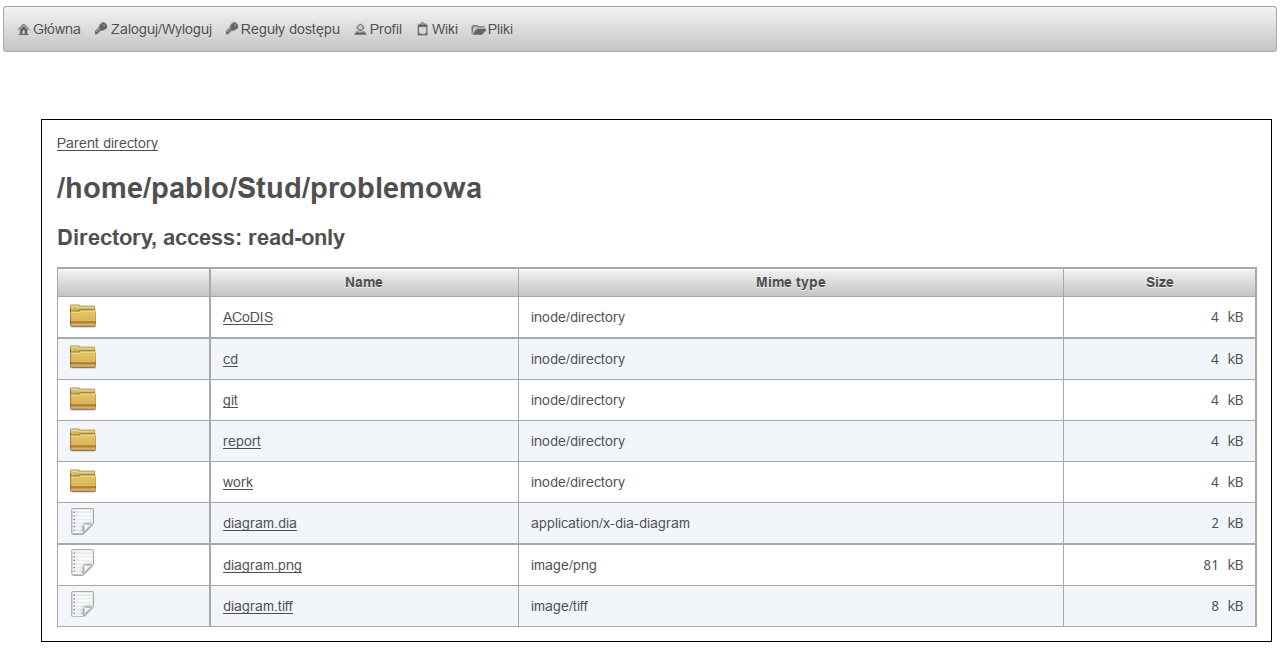
\includegraphics[width=\textwidth]{pictures/filebrowser/dir-ro.png}
\end{figure}

\begin{figure}[H]
  \caption{Przeglądanie pliku z prawami tylko do odczytu}
  \centering
    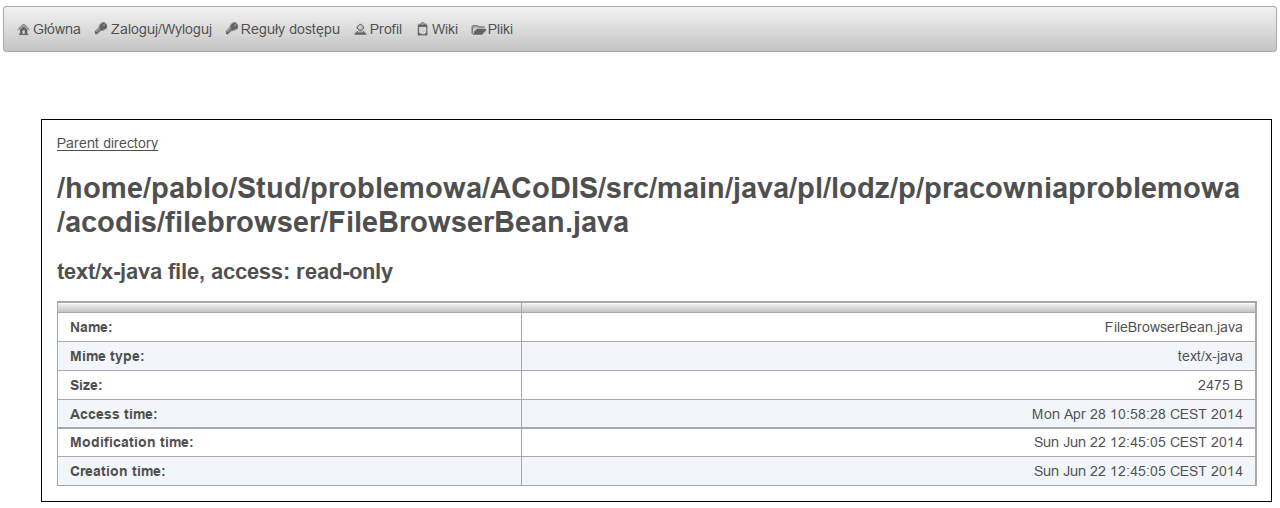
\includegraphics[width=\textwidth]{pictures/filebrowser/file-ro.png}
\end{figure}

Oczywiście aby jakiekolwiek informacje zostały wyświetlone, trzeba mieć przynajmniej uprawnienia
na poziomie \emph{read}. Dodatkową możliwością wspólną dla wszystkich typów węzłów
jest możliwość przejścia do węzła nadrzędnego. Wspomniane ,,przejście'' pomiędzy jednym
węzłem a drugim może oczywiście skończyć się informacją o braku uprawnień, w zależności
od tego jakie uprawnienia do węzła docelowego posiada dany użytkownik. Dla łatwości demonstracji
działania systemu, jeżeli nie jest sprecyzowane, jaki zasób ma być wyświetlony (w naszej aplikacji
dotyczy to tylko pierwszego uruchomienia komponentu), wybierany jest katalog domowy użytkownika,
który uruchamia serwer aplikacji.

\begin{figure}[H]
  \caption{Dodawanie nowych węzłów w katalogach z uprawnieniem \emph{write}}
  \centering
    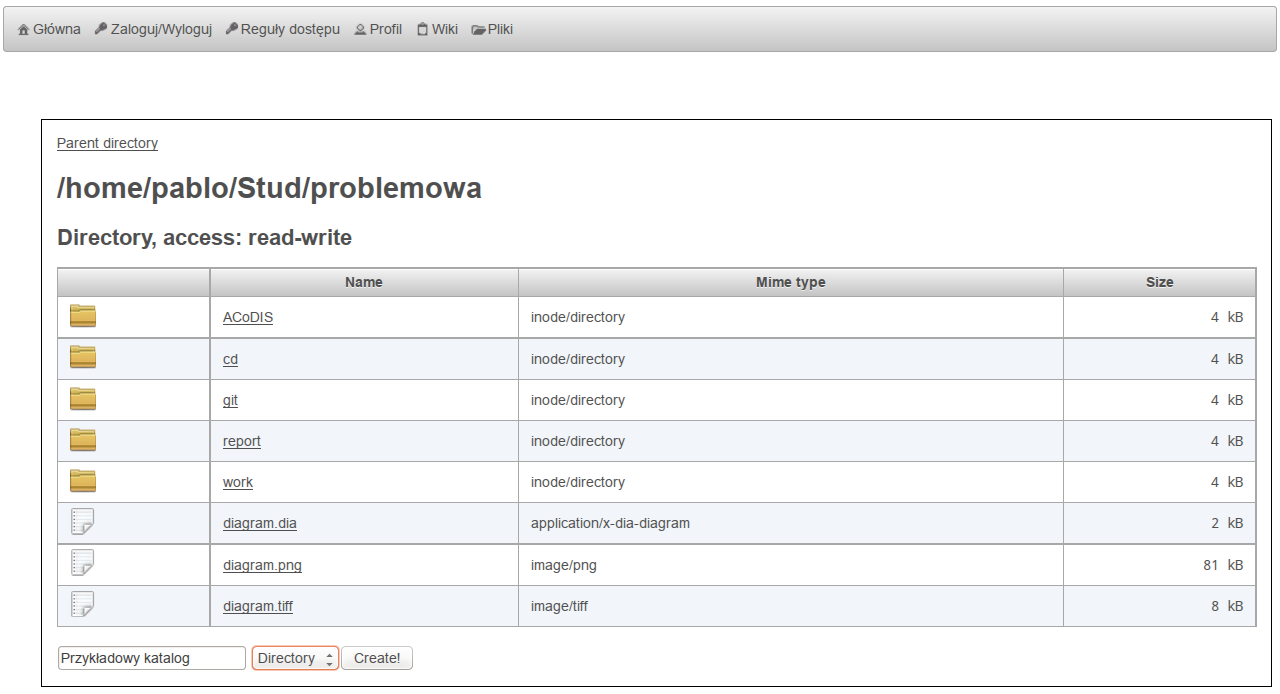
\includegraphics[width=\textwidth]{pictures/filebrowser/dir-rw1.png}
\end{figure}

\begin{figure}[H]
  \caption{Usuwanie pustych katalogów uprawnieniem \emph{write}}
  \centering
    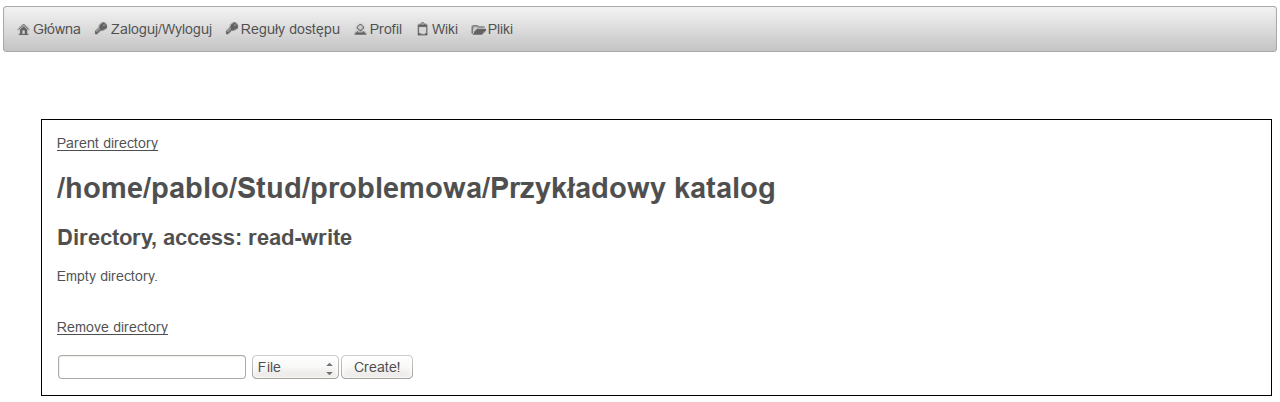
\includegraphics[width=\textwidth]{pictures/filebrowser/dir-rw2.png}
\end{figure}

Dodatkowe możliwości pojawiają się gdy uprawnienia do danego zasobu mają poziom \emph{write}.
Wtedy dla plików i pustych folderów pojawia się możliwość usunięcia bieżącego węzła,
oraz dla folderów (niezależnie od tego czy są puste czy nie) pojawia się możliwość
tworzenia pustych plików oraz pustych folderów wewnątrz nich.

\vspace\baselineskip

Podobnie jak we wszystkich pozostałych elementach naszej implementacji systemu ACoDIS, uprawnienia
te mogą z być specyficzne dla danego użytkownika lub wynikać z~jego roli oraz dodatkowo
zależeć od ścieżki do danego zasobu oraz wszelkiego rodzaju czynników zmieniających
się w sposób dynamiczny. Klasycznym przypadkiem jest tutaj upływający czas (i jedna z reguł
demonstrujących możliwości systemu jest oparta właśnie na tym).

\vspace\baselineskip

\subsubsection{Zaawansowane reguły dostępu i dynamizm}

Jak zostało wspomniane w ogólnym opisie modułu \texttt{filebrowser}, za każdym
razem odczytywana jest aktualna informacja o serwerowym systemie plików.
Zważywszy że struktura tego systemu plików może ulegać ciągłym zmianom
(między innymi wynikającym z działań użytkowników posiadających uprawnienia
na poziomie \emph{write} do pewnych węzłów), sam ten fakt czyni zachowanie
niniejszego moduły dynamicznym. Kluczowy jest jednak dla nas dynamizm
zdefiniowany wprost poprzez reguły dostępu -- opisany poniżej przykład 3. realizuje
tę myśl w sposób specyficzny dla modułu \texttt{filebrowser}.

\vspace\baselineskip

Przykładowe zaawansowane reguły związane z niniejszym modułem to:
\begin{enumerate}
\item Użytkownik posiada dostęp na poziomie \emph{write} do każdego
węzła, którego nazwa zaczyna się od jego loginu. O ile teoretycznie
można sobie wyobrazić system uprawnień
do plików w którym możemy dawać prawa do edycji zasobu pojedynczym
innym użytkownikom poprzez ustawienie odpowiedniej nazwy, to
rozwiązanie takie trudno nazwać optymalnym. Celem stworzenia tej
reguły jest jednak pokazanie, że możliwości takie jak niniejsza
mogą być wprowadzane do naszego systemu za pomocą pojedynczych
linijek kodu w języku Prolog.

\vspace\baselineskip

\item Użytkownik posiada dostęp na poziomie \emph{read} do każdego 
węzła, który posiada przodka o nazwie zaczynającej się od jego loginu.
Tak zdefiniowana reguła może zostać w praktycznym zastosowaniu przetłumaczona
na to, że każdy użytkownik ma dostęp przynajmniej na poziomie \emph{read}
do całej zawartości swojego katalogu domowego.

\vspace\baselineskip

\item Dla stworzonego na potrzeby demonstracji użytkownika \texttt{test3}
definiowaliśmy reguły dostępu polegające na tym, że użytkownik ten
może czytać wszystkie pliki na serwerze, oraz dodatkowo posiada
uprawnienie na poziomie \emph{write} do plików, które zostały utworzone
nie dawniej niż \(60\,\mbox{s}\) przed bieżącą chwilą. Reguła ta
w dosłowny sposób realizuje dynamizm systemu uprawnień, a także
ma największy potencjał jeżeli chodzi o zastosowania praktyczne --
nietrudno wyobrazić sobie system, w którym użytkownik po dodaniu
nowego zasobu ma pewien ograniczony czas na wycofanie się z~tego
i usunięcie go. Aby to uzyskać, można wykorzystać zaprojektowaną
przez nas regułę nawet bez wprowadzania do niej zmian, gdyż
stanowiące osobne zagadnienie ograniczenia
polegające na tym żeby użytkownik mógł usuwać tylko pliki
zamieszczone przez siebie mogłyby być realizowane przez
oddzielne reguły.
\end{enumerate}

\subsection{Komponent login}

\subsection{Komponent profile}
Komponent służy do przeglądania oraz edycji znajdujących się w systemie danych o użytkownikach. Jego implementację można podzielić logicznie na trzy modelowe warstwy: prezentacji, logiki i danych. \\
Warstwa prezentacji to utworzony z pomocą JSF front-end w postaci plików \textit{*.xhtml} zgromadzonych w folderze \textit{profile} komponentu. Znajdują się tam wszystkie elementy istotne dla działania komponentu, każdy z nich posiada strukturę umożliwiającą kontrolę dostępu opisaną w poprzednich rozdziałach. Do najważniejszych jego elementów należą \textit{profileReader} odpowiedzialny za wyświetlanie danych dostępnych tylko dla użytkowników z prawami do czytania treści oraz \textit{profileEditor} wprowadzający dodatkową funkcjonalność dla posiadaczy praw do zapisu. Pozostałe elementy agregują dodatkowe treści udostępniane w przeglądarce profili, tj. komunikaty wyświetlane użytkownikom i dodatkowe informacje o kontach. \\
Logika komponentu opiera się o pakiet \textit{pl.lodz.p.pracowniaproblemowa.acodis.profile} napisany w technologii Java. Składa się on z trzech klas:
\begin{itemize}
  \item \textit{Profile} - zawiera model danych dotyczący pojedynczego profilu. Definiuje wszystkie pola opisujące dane profilu oraz metody do obsługi tych danych.
  \item \textit{ProfileDataBean} - klasa przechowuje wszystkie dane które zmieniają się dynamicznie wraz z użytkowaniem systemu. Przechowuje listę wszystkich profili, aktualnie wyświetlany profil, odniesienie do danych użytkownika wykorzystanych do logowania oraz stan wyświetlanego aktualnie profilu. W metodach klasy kryją się funkcje odpowiedzialne za odczyt i zapis z warstwy danych oraz operacje odczytu i dokonania zmian stanu przeglądarki profili oraz samych danych.
  \item \textit{ProfileConverter} - z uwagi na to, że przeglądarka danych posiada listener ustawiony na element \textit{selectOneMenu} służacy do wyboru pożądanego profilu zaistniała potrzeba implementacji konwertera skupionego wprost na klasie \textit{Profile}. Zatem w klasie \textit{ProfileConverter} znajduje się kod implementujący inferfejs \textit{Converter}, służący do skutecznego porównania i wyboru odpowiednich instancji profili. Dzięki temu możliwa jest transformacja danych w postaci stringów z front-endu do obiektów Javy i na odwrót.
\end{itemize}
Warstwa danych składa się z pliku \textit{profiles.xml} znajdującego się w folderze zasobów systemu. Służy on za podręczną bazę wiedzy zaczytywaną do komponentu profili przy użyciu odpowiednich metod z klasy \textit{ProfileDataBean}. Jest to wydajny i przenośny sposób na agregację danych o użytkownikach, jednocześnie nie rzutujący na eskalację rozmiarów systemu. Jednocześnie rozwiązanie to jest łatwo wymienialne na inne technologie wraz z rozwojem i zmianami w systemie. \\
Komponent profili z perspektywy użytkowej składa się w zasadniczej mierze z elementu\textit{selectOneMenu} służącego do wyboru pożądanego profilu oraz obszaru wyświetlania danych o wybranej pozycji. Użytkownikowi z prawami \textit{write} została udostępniona dodatkowa funkcjonalność edycji danych wyświetlanego profilu, która jest obsługiwana za pomocą przycisków "edytuj", "zapisz" oraz "anuluj" wyświetlanych przy właściwych stanach przeglądarki profili. Dzięki zaimplementowanym mechanizmom komponent reaguje dynamicznie na aktualny stan warstwy danych oraz uzależnia sposób swojej reakcji od czasu oraz zalogowanego aktualnie użytkownika.

\subsection{Komponent security}
\subsection{Komponent wiki}

Poniżej prezentujemy przykładowe zaimplementowane przez nas reguły dostępowe:
\begin{verbatim}

isPasswordFor('test','test').
isPasswordFor('no','no').
isPasswordFor('read','read').
isPasswordFor('write','write').
isPasswordFor('admin','admin').
isPasswordFor('zenek','zenek').
isPasswordFor('franek','franek').

hasRole('admin','administrators').
hasRole('zenek','wikipedists').
hasRole('franek','fileadmins').

hasRole(Username,'wikipedists') :- hasRole(Username, 'administrators').
hasRole(Username,'fileadmins') :- hasRole(Username, 'administrators').

canAccessAtIfLogged(user('read','read'),_, readAccess).
canAccessAtIfLogged(user('write','write'),_, writeAccess).

roleCanAccessAtIfLogged('administrators',_, writeAccess).
\end{verbatim}

\section{Oprawa wizualna}
Do Stworzenia oprawy wizualnej, wykorzystany został framework JSF i biblioteka komponentów PrimeFaces. JSF umożliwia tworzenie szablonów, wykorzystywanych później przez strony komponentów. Primefaces dostarcza wielu użytecznych komponentów, gotowych do wykorzystania, jak na przykład menu, rozwijane panele, czy okienka powiadomień.\\
Główny moduł strony składa się z następujących elementów:
\begin{itemize}
  \item nagłówka, w którym znajduje się menu, umożliwiające nawigację do stron poszczególnych komponentów 
  \item stopki, nie pełniącej żadnej kluczowej funkcji, ale ładnie dopełniającej kompozycję strony
  \item części środkowej, wyświetlającej zawartość strony komponentu
  \item opcjonalnego, rozwijanego panelu bocznego, wyświetlanego w miarę potrzeby (gdy jest sens użycia go w komponencie)
\end{itemize}
Oczywiście, w razie potrzeby, można dodawać kolejne elementy, a nawet je zagnieżdżać (przykładem zagnieżdżenia jest lewy panel, stanowiący fragment środkowej części strony, dzięki czemu nie nachodzi on na nagłówek i stopkę).\\
Wykorzystanie wspomnianego wyżej panelu bocznego jest widoczne w komponencie Wikipedii. Znajdują się na nim linki, umożliwiające tworzenie i zarządzanie zawartością wikipedii, a także drzewko zawartości strony (kategorie i artykuły). Wyodrębnienie tych elementów ze strony głównej pozwala na wygodniejszą i efektywniejszą nawigację i zarządzanie stroną. Boczne menu jest skalowalne, w związku z czym można je dopasować do indywidualnych potrzeb. Istnieje też opcja zwinięcia go, co umożliwia wyświetlanie treści na niemal całej szerokości strony.\\
Innymi przykładami wykorzystania komponentów PrimeFaces są rozwijane obszary informacji o autorach projektu, widoczne na stronie głównej, czy też okienka informacyjne, powiadamiające o braku uprawnień do przeglądania określonych treści. W tym drugim przypadku widać możliwości konfiguracyjne komponentów PrimeFaces. Tutaj, do okienka informacyjnego, zostało też dodane wyciemnienie tła, uniemożliwiające interakcję ze stroną aż do momentu zamknięcia okna powiadomienia.

\section{Dyskusja rozwiązania i podsumowanie}
Nasze rozwiązanie postawionego problemu uznajemy za udane. Jednakże gdybyśmy następnym razem wykonywali podobny projekt, to nie zastosowalibyśmy Javy, ani tym bardziej technologii JSF.
Problemem technologii JSF jest jej stanowość. Przystępując do wykonania projektu i wybierając JavęEE i JSF kierowaliśmy się faktem, że wszyscy członkowie zespołu znają język Java 
i relatywnie łatwe będzie dla nich wdrożenie się w technologię JSF. Jednakża technologia ta nie spełniła pokładanych w niej oczekiwań. Jej głównym problemem jest fakt,
że każda odsłona strony powoduje wczytanie zapamiętanego na serwerze drzewa komponentów. Powoduje to, że komponenty te są statyczne i trudno było zmusić tą technologię do
dynamicznego podmieniania komponentów pomiędzy wyświetleniami strony. Udało się to w końcu zrealizować, ale dość wysokim kosztem. Dlatego w następnych podobnych projektach
nie wykorzystalibyśmy już Javy, ale bardziej dynamiczne środowiska np. Smalltalk i Seaside, Ruby on Rails lub Pythona i Django. 
\section{Udział w projekcie}
Pracami podzieliliśmy się w następujący sposób:
\begin{itemize}
\item Mateusz Grotek -- projekt systemu, zarządzanie uprawnieniami, Prolog
\item Mateusz Jakubczak -- komponent profili użytkownika
\item Rafał Jurkiewicz -- szablon strony i warstwa wizualna
\item Łukasz Kotyński -- komponent wikipedii
\item Paweł Tarasiuk -- komponent obsługi plików
\end{itemize}

\begin{thebibliography}{10}
\bibitem{owasp}Access Control Cheat Sheet \url{https://www.owasp.org/index.php/Access\_Control\_Cheat\_Sheet}
\bibitem{computer}Computer access control \url{http://en.wikipedia.org/wiki/Computer\_access\_control}
\bibitem{wikibooks}Access Control Systems w \textsl{Fundamentals of Information Systems Security} \texttt{http://en.wikibooks.org/wiki/\\Fundamentals\_of\_Information\_Systems\_Security/Access\_Control\_Systems}
\bibitem{TCSEC}Trusted Computer System Evaluation Criteria \url{http://en.wikipedia.org/wiki/Trusted\_Computer\_System\_Evaluation\_Criteria}
\bibitem{NIST}Role Based Access Control (RBAC) and Role Based Security \url{http://csrc.nist.gov/groups/SNS/rbac/}
\bibitem{RBAC}Ferraiolo, D. F., Kuhn, D.R., 1992. Role-Based Access Control. 15th National Computer Security Conference
\bibitem{NISTModel}Sandhu, R., Ferraiolo D., Kuhn R. 2000. The NIST Model for  Role Based Access Control:  Toward a Unified Standard. 
Proceedings, 5th ACM Workshop on Role Based Access Control, Lipiec 26--27, 2000, Berlin, pp. 47--63 
\bibitem{Drools}Drools -- The Business Logic integration Platform \url{https://www.jboss.org/drools/}
\bibitem{Prolog}Kluźniak F., Szpakowicz S. 1985. Prolog For Programmers.
\end{thebibliography}
\end{document}
